%
%   $Id$
%   This file is part of the FPC documentation.
%   Copyright (C) 2000 by Florian Klaempfl
%
%   The FPC documentation is free text; you can redistribute it and/or
%   modify it under the terms of the GNU Library General Public License as
%   published by the Free Software Foundation; either version 2 of the
%   License, or (at your option) any later version.
%
%   The FPC Documentation is distributed in the hope that it will be useful,
%   but WITHOUT ANY WARRANTY; without even the implied warranty of
%   MERCHANTABILITY or FITNESS FOR A PARTICULAR PURPOSE.  See the GNU
%   Library General Public License for more details.
%
%   You should have received a copy of the GNU Library General Public
%   License along with the FPC documentation; see the file COPYING.LIB.  If not,
%   write to the Free Software Foundation, Inc., 59 Temple Place - Suite 330,
%   Boston, MA 02111-1307, USA.
%
%%%%%%%%%%%%%%%%%%%%%%%%%%%%%%%%%%%%%%%%%%%%%%%%%%%%%%%%%%%%%%%%%%%%%
% The IDE
%%%%%%%%%%%%%%%%%%%%%%%%%%%%%%%%%%%%%%%%%%%%%%%%%%%%%%%%%%%%%%%%%%%%%
\chapter{The IDE}

The IDE (\textbf{I}ntegrated \textbf{D}evelopment \textbf{E}nvironment)
provides a comfortable user interface to the compiler. It contains an 
editor with syntax highlighting, a debugger, symbol browser etc. 
The IDE is a textmode application which has the same look and feel 
on all supported operating systems. It is modeled after the IDE of Turbo
Pascal, so many people should feel comfortable using it.

Currently, the IDE is available for \dos, \windows and \linux.

%%%%%%%%%%%%%%%%%%%%%%%%%%%%%%%%%%%%%%%%%%%%%%%%%%%%%%%%%%%%%%%%%%%%%%%
% First steps with the IDE
\section{First steps with the IDE}
%
% Starting the IDE
%
\subsection{Starting the IDE}
The IDE is started by entering the command:
\begin{verbatim}
fp
\end{verbatim}
at the command line. It can also be started from a graphical user 
interface such as \windows. 
\begin{remark}
Under \windows, it is possible to switch between windowed mode and 
full screen mode by pressing \key{Alt-Enter}).
\end{remark}
%
% IDE command-line options.
%
\subsection{IDE Command line options}
When starting the IDE, command line options can be passed:
\begin{verbatim}
fp [-option] [-option] ... <file name> ...
\end{verbatim}
\var{Option} is one of the following switches (the option letters
are case insensitive):
\begin{description}
\item [-N] (\dos only) Do not use long file names. \windows 95 and later
versions of \windows provide an interface to DOS applications to access 
long file names. 
The IDE uses this interface by default to access files. Under certain 
circumstances, this can lead to problems. This switch tells the IDE not to
use the long filenames.
\item [-Cfilename] This option, followed by a filename, tells the IDE to
read its options from \file{filename}. There should be no whitespace between
the file name and the \var{-C}.
\item [-R] After starting the IDE, it changes automatically to the directory
which was active when the IDE exited the last time.
\end{description}
The files given at the command line are loaded into edit
window automatically.

\begin{remark}
Under DOS/Win32, a \var{/} can be used instead of \var{-} to pass a
command line switch to the IDE.
\end{remark}

\subsection{The IDE screen}

After start up, the screen of the IDE looks like 
\begin{htmlonly}
this:
\htmladdimg{../pics/idestart.gif}
\end{htmlonly}
\begin{latexonly}
figure \ref{fig:idestart}.
\begin{figure}
\caption{The IDE screen immediatly after startup}
\label{fig:idestart}
\ifpdf
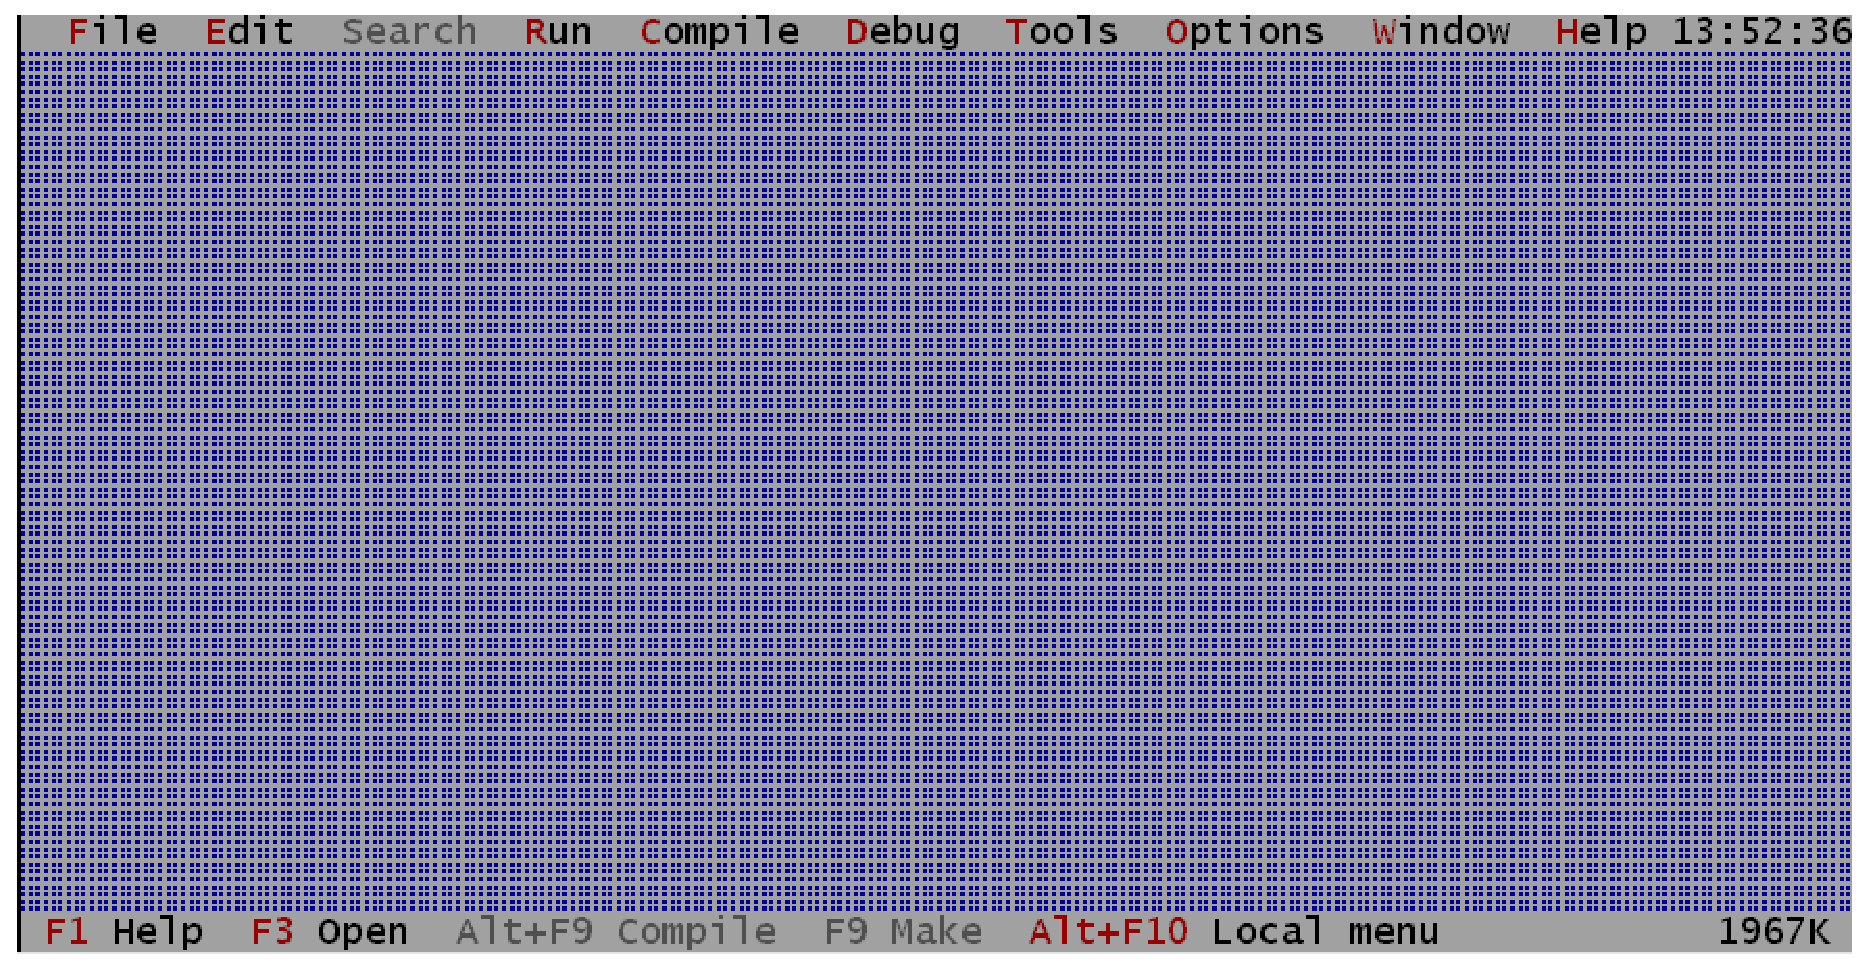
\epsfig{file=pics/idestart.png,width=\textwidth}
\else
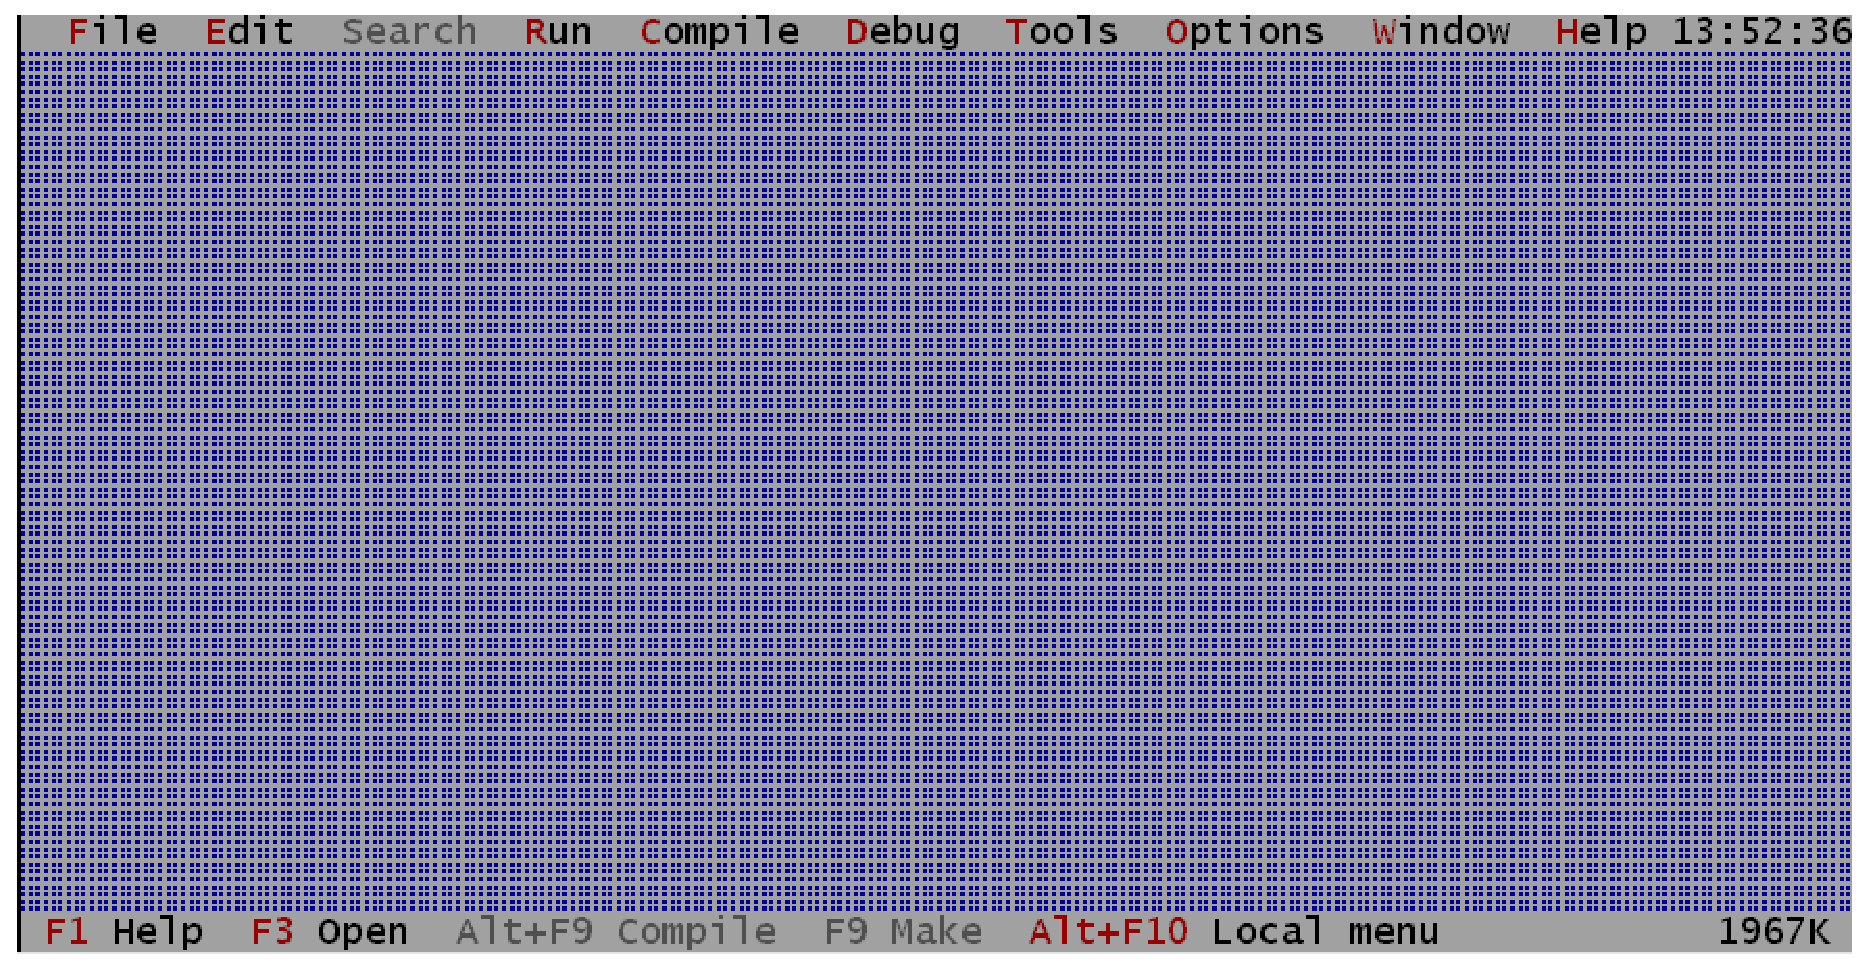
\epsfig{file=pics/idestart.eps,width=\textwidth}
\fi
\end{figure}
\end{latexonly}
At top of the screen the \emph{menu bar} is visible, at the bottom
the \emph{status bar}. The empty space between them is called the
\emph{desktop}.

The statusbar shows the keyboard shortcuts for frequently used 
commands, and allows quick access to these commands by clicking 
them with the mouse. 
At the right edge of the statusbar, the current amount of unused 
memory is displayed. This is only an indication, since the IDE 
tries to allocate more memory from the operating system if it 
runs out of memory.

The menu provides access to all of the IDE's functionality, and
at the right edge of the menu, a clock is displayed.

The IDE can be left by selecting \var{File|Exit} in the menu
\footnote{\var{File|Exit} means select the item Exit in the menu File}
or by pressing \key{Alt-X}.

%%%%%%%%%%%%%%%%%%%%%%%%%%%%%%%%%%%%%%%%%%%%%%%%%%%%%%%%%%%%%%%%%%%%%%%
% Navigating in the IDE
\section{Navigating in the IDE}
The IDE can be navigated both with the keyboard and with a mouse, if your
system has a mouse.

\subsection{Using the keyboard} 
All functionality of the IDE is available through use of the keyboard.
\begin{itemize}
\item It is used for typing and navigating through the sources.
\item Editing commands such as copying and pasting text.
\item Moving and resizing windows.
\item It can be used to access the menu, by pressing \key{ALT} and the
appropriate highlighted menu letter, or by pressing \key{F10} and
navigating through the menu with the arrow keys.

more information on the menu can be found in \sees{idemenu}
\item Many commands in the IDE are bound to shortcuts, i.e. typing a special
combination of keys will execute a command immediatly.
\end{itemize}
\begin{remark}
A complete reference of all keyboard shortcuts can be found in
\sees{keyshortcuts}.
\end{remark}

\subsection{Using the mouse}
\label{suse:mouseusage}
If the system is equipped with a mouse, it can be used to work with the
IDE. The left button is used to select menu items, press buttons, select
text blocks etc. 

The right mouse button is used to access the local menu, if
it is available. Holding down the \key{Ctrl} or \key{Alt} key and 
clicking the right button will execute user defined functions, 
see \sees{prefmouse}.

\begin{remark}
\begin{enumerate}
\item Occasionally, the manual uses the term "drag the mouse". This
means that the mouse is moved while the left mouse button is being 
pressed.
\item 
The action of mouse buttens may be reversed, i.e. the actions of the left
mouse button can be assigned to the right mouse button and vice versa  
\footnote{See \sees{prefmouse} for more information on how to reverse the
actions of the mouse buttons.}. Throughout the manual, it is assumed 
that the actions of the mouse buttons are not reversed.
\item
The mouse is not allways available, even if a mouse is installed:
\begin{itemize}
\item The IDE is running under \linux throught a telnet connection from 
a \windows machine.
\item The IDE is running under \linux in an X-term under X-windows.
\end{itemize}
\end{enumerate}
\end{remark}

%%%%%%%%%%%%%%%%%%%%%%%%%%%%%%%%%%%%%%%%%%%%%%%%%%%%%%%%%%%%%%%%%%%%%%%
% Windows
\section{Windows}
\label{se:windows}
Nowadays, working with windowed applications should be no problem for
most \windows and \linux users. Nevertheless, the following section 
describes how the windows work in the \fpc IDE, to allow efficient 
work with it.
%
% Window basics
%
\subsection{Window basics}
\label{se:windowbasics}
\begin{htmlonly}
A common IDE window is displayed  below:
\htmladdimg{../pics/idewin.gif}
\end{htmlonly}
\begin{latexonly}
A common IDE window is displayed in figure \ref{fig:idewin}.
\begin{figure}
\caption{A common IDE window}
\label{fig:idewin}
\ifpdf
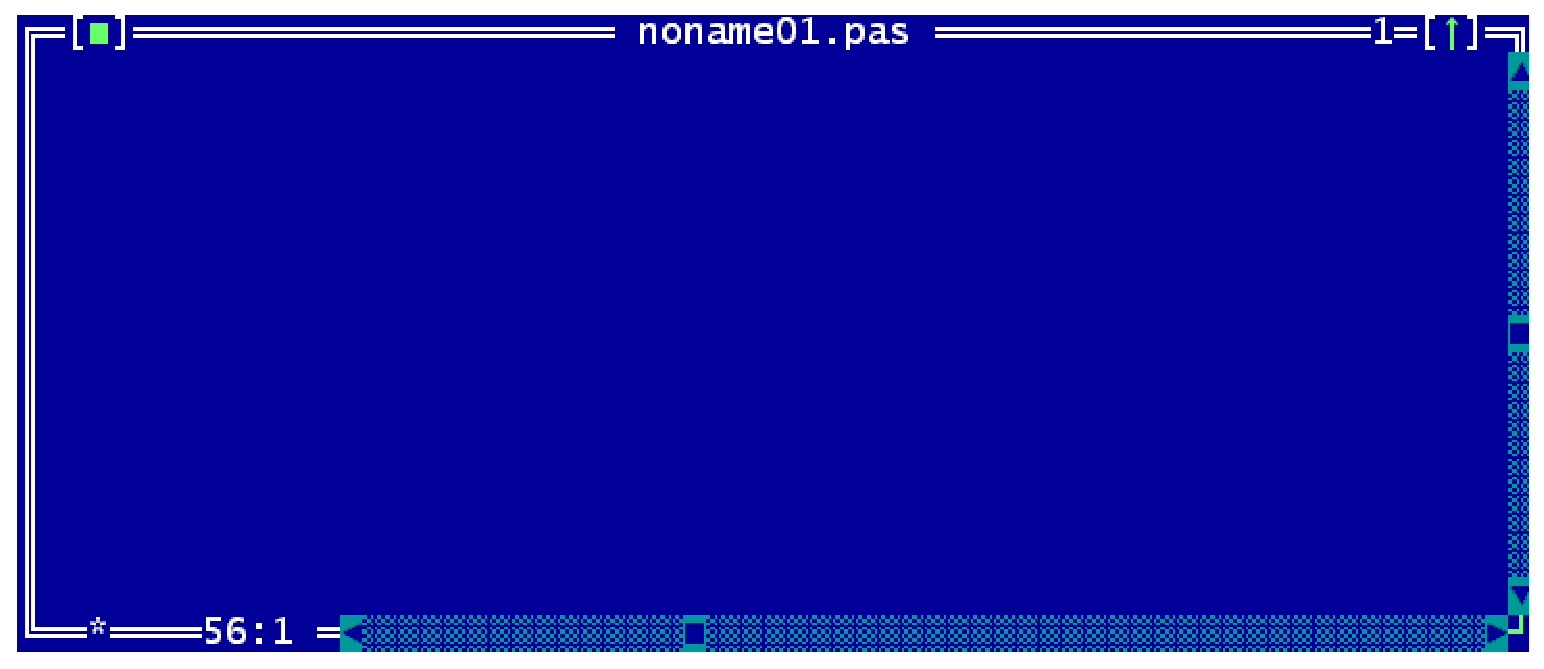
\epsfig{file=pics/idewin.png,width=\textwidth}
\else
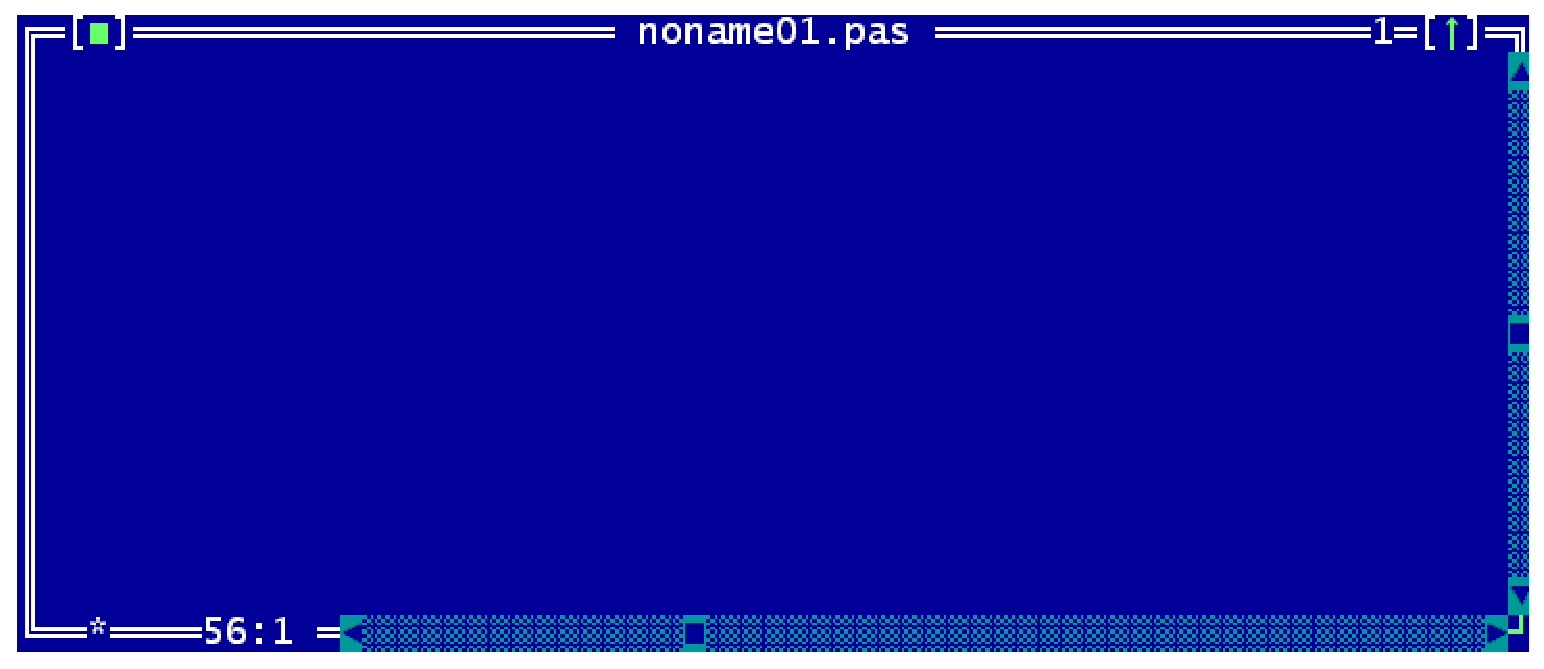
\epsfig{file=pics/idewin.eps,width=\textwidth}
\fi
\end{figure}
\end{latexonly}
The window is surrounded by a so-called \emph{frame}, the white double
line around the window. 

At the top of the window 3 things are displayed:
\begin{itemize}
\item 
At the upper left corner of the window, a \emph{close icon} is shown. 
When clicked, the window will be closed. It can be also closed by
 pressing \key{Alt-F3} or selecting the menu item \var{Window|Close}. 
All open windows can be closed by selecting the menu item 
\var{Window|Close all}.
\item In the middle, the title of the window is displayed.
\item At the upper right corner, a small green arrow is visible.
Clicking this arrow zooms the window so it covers the whole desktop. 
Clicking this arrow on a zoomed window will restore old size of the 
window. Pressing the key \key{F5} has the same effect as clicking 
that arrow. The same effect can be achieved with the menu item \var{Window|Zoom}.
Windows and dialogs which aren't resizeable can't be zoomed, either.
\end{itemize}

The right edge and bottom edges of a window contain scrollbars.
They can be used to scroll the window contents with the mouse. 
The arrows at the ends of the scrollbars can be clicked to scroll the 
contents line by line. Clicking on the dotted area between the arrows 
and the cyan-coloured rectangle will scroll the window's content 
page by page. By dragging the rectangle the content can be scrolled 
continuously.

The star and the numbers in the lower left corner of the window
display information about the contents of the window. They
are explained in the section about the editor, see \sees{editingtext}.

%
% Sizing+moving windows
%
\subsection{Sizing and moving windows}
\label{se:windowsizingmoving}
A window can be moved and sized using the mouse and the keyboard:
To move a window, either:
\begin{itemize}
\item using the mouse, click on the title bar and drag the window 
with the mouse.
\item using the keyboard, go into the size/move mode
by pressing \key{Ctrl-F5} or selecting the menu item
\var{Window|Size/Move}. . Using the cursor keys the window can be moved. 
The size/move mode can be left by pressing \key{Enter}. 
In this case, the window will keep its size and position. 
Alternativly, pressing \key{Esc} will restore the old position.
\end{itemize} 
To resize a window, either:
\begin{itemize}
\item using the mouse, click on the lower right corner of the window
and drag it.
\item using the keyboard, go into the size/move mode
by pressing \key{Ctrl-F5} or selecting the menu item
\var{Window|Size/Move}. The window frame will be green to indicate that
the IDE is in size/move mode. 
By pressing shift and the cursor keys simultaneously, the window can 
be resized.  The size/move mode can be left by pressing
\key{Enter}. In this case, the window will keep the new size.
Pressing \key{Esc} will restore the old size.
\end{itemize}
Not all windows can be resized. This applies, for example, to
\emph{dialog windows} (\sees{dialogwindow}).

A window can also be hidden. To hide a window, the \key{Ctrl-F6} key
combination can be used, or the \var{Window|Hide} menu may be selected.
To restore a Hidden window, it is necessary to select it from the window
list. More information about the window list can be found in the next
section.   
%
% Multiple windows
%
\subsection{Working with multiple windows}
\label{se:multiplewindows}
When working with larger projects, it is likely that multiple windows 
will appear on the desktop. However, only one of these windows will be 
the active window, all other windows will be inactive.

An inactive window is identified by a grey frame. An inactive window can
be made active in one of several ways:
\begin{itemize}
\item using the mouse, activate a window by clicking on it.
\item using the keyboard, pressing \key{F6} will step trough all open 
windows. To activate the previously activated window, \key{Shift-F6} can
be used.
\item the menu item \var{Window|Next} can be used to activate the next 
window in the list of windows, while \var{Window|Previous} will select
the previous window.
\item If the window has a number in the upper right corner, it can be
activated by pressing \key{Alt-<number>}.
\item Pressing \key{Alt-0} will pop up a dialog with a lis  with all 
available windows which allows a quick activation of windows which 
don't have a number.
\end{itemize}

The windows can be ordered and placed on the IDE desktop by zooming and
resizing them with the mouse or keyboard. This is a tyime-consuming task, 
and particularly difficult with the keyboard. Instead, the menu items
\var{Window|Tile} and \var{Window|Cascade} can be used:
\begin{description}
\item[Tile] will divide whole desktop space evenly between all resizable 
windows. 
\item[Cascade] puts all windows in a cascaded position. 
\end{description}

In very rare cases the screen of the IDE may be mixed up. In this
case the whole IDE screen can be refreshed by selecting the menu item 
\var{Window|Refresh display}.
%
% Dialog windows
%
\subsection{Dialog windows}
\label{se:dialogwindow}
In many cases the IDE displays a dialog window to get user input.
The main difference to normal windows is that other windows cannot be
activated while a dialog is active. Also the menu is not accessible while in
a dialog. This behavior is called \emph{modal}. To activate another window, 
the modal window or dialog must be closed first.

\begin{htmlonly}
A typical dialog window looks like:
\htmladdimg{../pics/idedlg.gif}
\end{htmlonly}
\begin{latexonly}
Figure \ref{fig:idedlg} shows a typical dialog window.
\begin{figure}
\caption{A typical dialog window}
\label{fig:idedlg}
\ifpdf
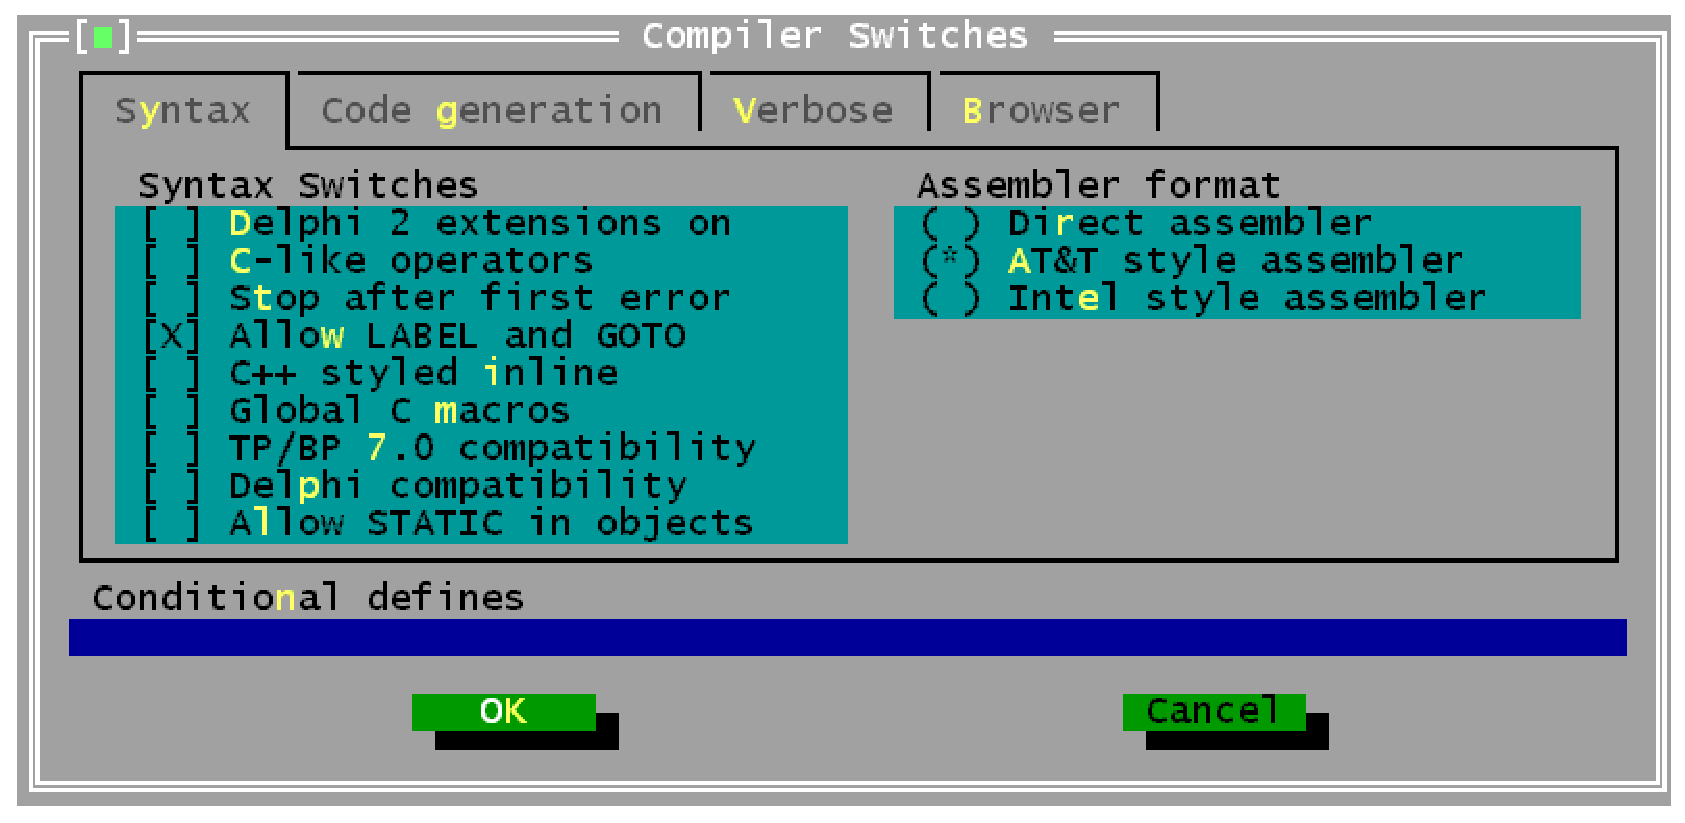
\epsfig{file=pics/idedlg.png,width=\textwidth}
\else
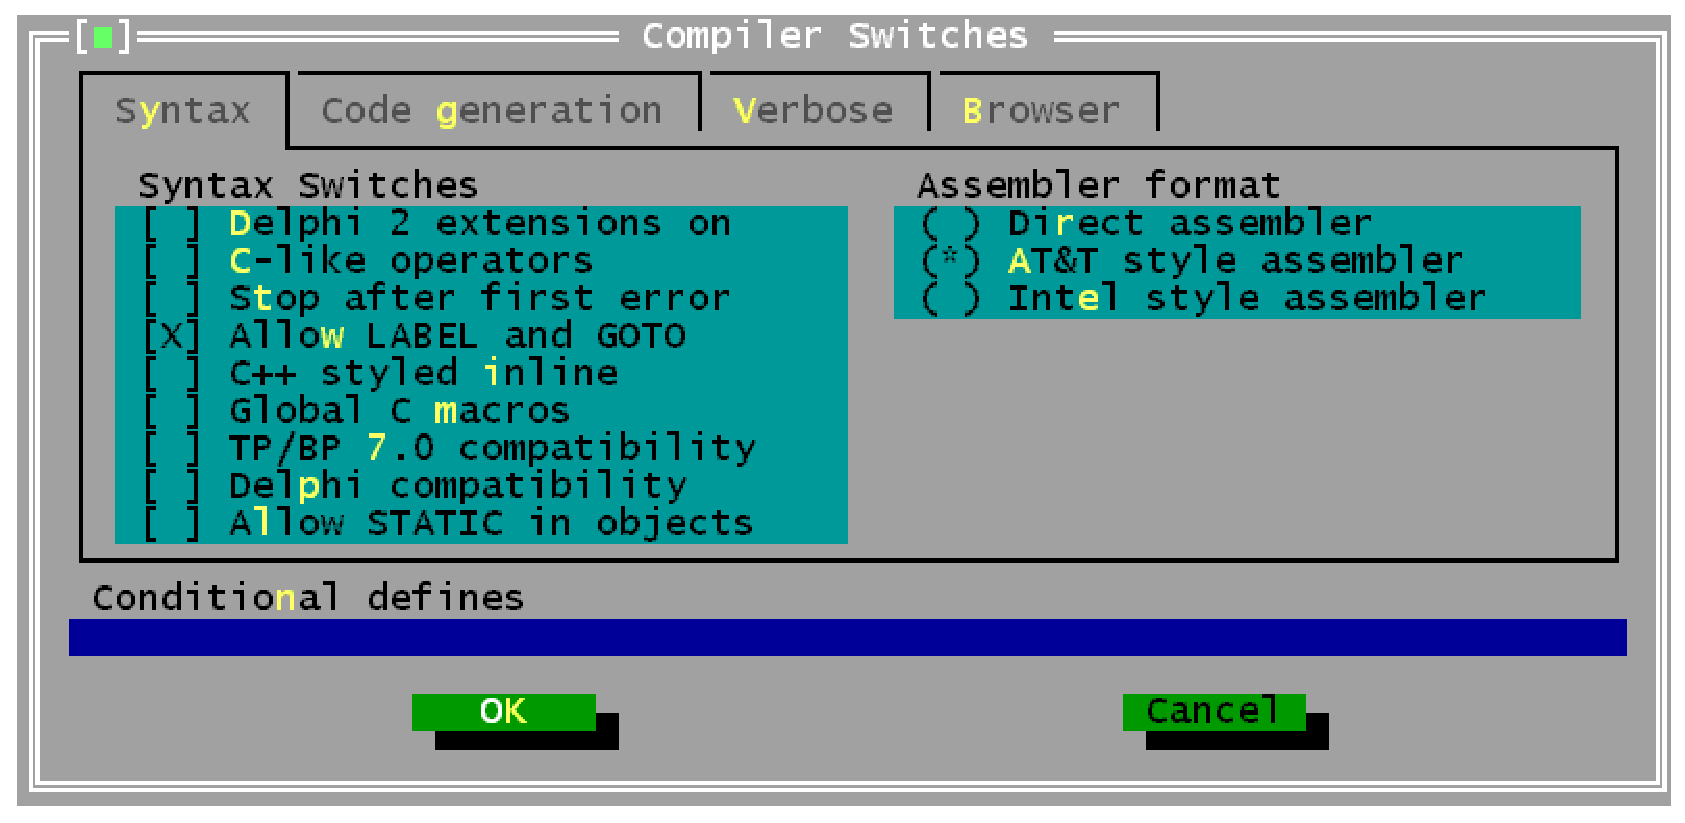
\epsfig{file=pics/idedlg.eps,width=\textwidth}
\fi
\end{figure}
\end{latexonly}

%%%%%%%%%%%%%%%%%%%%%%%%%%%%%%%%%%%%%%%%%%%%%%%%%%%%%%%%%%%%%%%%%%%%%%%
% The menu
\section{The Menu}
\label{se:idemenu}
The main menu (the gray bar at the top of the IDE) provides access to all the
functionality of the IDE. It also displays a clock, displaying the current
time. The menu is always available, except when a dialog is opened. If a
dialog is opened, it must be closed first in order to access the menu.

In certain windows, a local menu is also available. The local menu will
appear where the cursor is, and provides additional commands that are 
context-sensitive.
%
% Accessing the menu
%
\subsection{Accessing the menu}
The menu can be accessed in a number of ways:
\begin{enumerate}
\item By using the mouse to select items. The mouse cursor should be located
over the desired menu item, and a left mouse click will then select it.
\item By pressing \key{F10}. This will switch the IDE focus to the menu. 
Use the arrow keys can then be used to navigate in the menu, the 
\key{Enter} key should be used to select items.
\item To access menu items directly, \key{Alt-<highlighted menu letter>}
can be used to select a menu item. Afterwards submenu entries can be selected 
by pressing the highlighted letter, but without \key{Alt}. 
E.g. \key{Alt-S G} is a fast way to display the \emph{goto line} dialog.
\end{enumerate}
Every menu item is explained by a short text in the status bar.

When a local menu is available, it can be accessed by pressing
the right mouse button or \key{Alt-F10}. 

In the subsequent, all menu entries and their actions are described.
%
% The file menu
%
\subsection{The File menu}
\label{se:menufile}
\begin{description}
\item[New] Opens a new, empty editor window. 
\item[New from template] Prompts for a template to be used, asks to fill in
any parameters, and then starts a new editor window with the template.
\item[Open] (\key{F3}) Presents a file selection dialog, and opens 
the selected file in a new editor window. 
\item[Save] (\key{F2}) Saves the contents of the current edit window 
with the current filename. If the current edit window does not yet have
a filename, a dialog is presented to enter a filename.
\item[Save as] Presents a dialog in which a filename can be entered. The
current window's contents are then saved to this new filename, and the
filename is stored for further save actions.
\item[Change dir] Presents a dialog in which a directory can be selected.
The current working directory is then changed to the selected directory.
\item[Dos shell] executes a command shell. After the shell exited, the
IDE resumes.
\item[Exit] (\key{ALT-X}) Exits the IDE. If any unsaved files are 
in the editor, the IDE will ask if these files should be saved.
\end{description}
%
% The edit menu
%
\subsection{The Edit menu}
\label{se:menuedit}
\begin{description}
\item[Undo] (\key{ALT-BkSP})
Undo the last editing action. The editing actions are stored in a buffer,
selecting this mechanism will move backwards through this buffer, i.e.
multiple undo levels are possible.
\item[Redo] Redo the last action that was previously undone. Redo can redo
multiple undone actions. 
\item[Dump undo]
Clears the undo buffer. After this action, the undo and redo menu will be 
unavailable till new editing actions have taken place.
\item[Undo all]
Undo all actions in the undo buffer. If a new empty file was started, this
action should clear the window contents again.
\item[Redo all]
Redo all editing actions that were undone.
\item[Cut] (\key{Shift-DEL}) Copy the current selection to the clipboard
and delete the selection from the text. Any previous clipboard contents is
lost after this action. After this action, the clipboard contents can be 
pasted elsewhere in the text.
\item[Copy] (\key{Ctrl-INS}) Copy the current selection to the clipboard.
Any previous clipboard contents is lost after this action. 
After this action, the clipboard contents can be pasted elsewhere in the text.
\item[Paste] (\key{Shift-INS}) Insert the current clipboard contents in
the text at the cursor position. The clipboard contents remains as it was.
\item[Clear] (\key{Ctrl-DEL}) clears (i.e. deletes) the current
selection.
\item[Show clipboard] Opens a window in which the current clipboard contents
is shown.
\end{description}
%
% The Search menu
%
\subsection{The Search menu}
\label{se:menusearch}
\begin{description}
\item[Find] (\key{Ctrl-Q F}) presents the search dialog. A search text 
can be entered, and when the dialog is closed, the entered text is searched
in the active window. If the text is found, it will be selected. 
\item[Replace] (\key{Ctrl-Q A} presents the search and replace dialog.
After the dialog is closed, the search text will be replaced by the replace
text in the active window.
\item[Search again] (\key{CTRL-L}) repeats the last search or search and replace action,
 using  the same parameters.
\item[Go to line number] (\key{Alt-G}) prompts for a line number, and
then jumps to this line number.
\item[Find procedure]
Not yet implemented.
\item[Objects]
Not yet implemented.
\item[Modules]
Not yet implemented.
\item[Globals]
Not yet implemented.
\item[Symbol]
Not yet implemented.
\end{description}
%
% The Run menu
%
\subsection{The Run menu}
\label{se:menurun}
\begin{description}
\item[Run] (\key{Ctrl-F9})
If the sources were modified, compile the program. If the compile is
successful, the program is executed. If the primary file  was set, then 
that is used to determine which program to execute. See \sees{menucompile}
for more information on how to set the primary file.
\item[Step over] (\key{F8})
Run the program till the next source line is reached. If any calls to 
procedures are made, these will be executed completely as well.
\item[Trace into] (\key{F7})
Execute the current line. If the current line contains a call to another
procedure, the process will stop at the entry point of the called procedure.
\item[Goto cursor] (\key{F4})
Runs the program till the execution point matches the line where the cursor
is.
\item[until return]
Runs the current procedure till it exits.
\item[parameters]
This menu item allows to enter parameters that will be passed on to the
program when it is being executed.
\item[program reset] (\key{Ctrl-F2}) if the program is being run or 
debugged, the debug session is aborted, and the running program is killed.
\end{description}
%
% The compile menu
%
\subsection{The Compile menu}
\label{se:menucompile}
\begin{description}
\item[Compile] (\key{Alt-F9}) Compiles the contents of the active window.  
If the primary file was set, the primary file is compiled instead.
\item[Make] (\key{F9}) Compiles the contents of the active window, and
any files that the unit or program depends on and that were modified since
the last compile.
If the primary file was set, the primary file is compiled instead.
\item[Build]
Compiles the contents of the active window, and any files that the unit or 
program depends on, whether they were modified or not.
If the primary file was set, the primary file is compiled instead.
\item[Target] Sets the target operating system for which should be compiled. 
\item[Primary file] Sets the primary file. If set, any run or compile command 
will act on the primary file instead of on the active window. The primary
file need not be loaded in the IDE for this to have effect.
\item[Clear primary file]
Clears the primary file. After this command, any run or compile action will
act on the active window.
\item[Information] Displays some information about the current program.
\item[Compiler messages] (\key{F12}) displays the compiler messages
window. This window will display the messages generated by the compiler
during the last compile.
\end{description}
%
% The debug menu
%
\subsection{The Debug menu}
\label{se:menudebug}
\begin{description}
\item[Output]
\item[User screen] (\key{Alt-F5}) switches to the screen as it was last
left by the running program.
\item[Breakpoint] (\key{Ctrl-F8})
Sets a breakpoint at the current line. When debugging, program execution
will stop at this breakpoint.
\item[Call stack] (\key{Ctrl-F3})
Shows the call stack. The call stack is the list of addresses (and
filenames and line numbers, if this information was compiled in) of 
procedures that are currently being called in the running program.
\item[Registers]
Shows the current content of the CPU registers. 
\item[Add watch] (\key{Ctrl-F7}) Add a watch. A watch is an expression
that can be evaluated by the IDE and shown in a special window. usually this
is the contents of some variable. 
\item[Watches]
Shows the current list of watches in a separate window.
\item[Breakpoint list]
Shows the current list of breakpoints in a separate window.
\item[GDB window]
Shows the GDB debugger console. This can be used to interact with the debugger
directly.
\end{description}
%
% The tools menu
%
\subsection{The Tools menu}
\label{se:menutools}
\begin{description}
\item[Messages] (\key{F11}) Show the messages window. 
This window contains the output from one of the tools. For more information,
see \sees{toolsmessages}.
\item[Goto next] (\key{Alt-F8}) goto next message.
\item[Goto previous] (\key{Alt-F7}) goto previous message
\item[Grep] (\key{SHIFT-F2}) Prompts for a regular expression and options
to be given to grep, and then executes \file{grep} with the given expression and
options. For this to work, the \file{grep} program must be installed on your
system, and be in a directory that is in the \var{PATH}. For more
information, see \sees{grep}.
\item[Calculator] 
Displays the calculator. For more information, see \sees{calculator}
\item[Ascii table] Displays the \var{ASCII} table. For more information, see
\sees{asciitable}
\end{description}
%
% The Search menu
%
\subsection{The Options menu}
\label{se:menuoptions}
\begin{description}
\item[Mode] Presents a dialog to set the current mode of the compiler. The
current mode is shown at the right of the menu entry. For more information,
see \sees{compilermode}.
\item[Compiler] Presents a dialog that can be used to set common compiler
options. These options will be used when compiling a program or unit.
\item[Memory sizes]
Presents a dialog where the stack size and the heap size for the program can
be set. These options will be used when compiling a program.
\item[Linker]
Presents a dialog where some linker options can be set. These options will
be used when a program or library is compiled.
\item[Debugger]
Presents a dialog where the debugging options can be stored. These options
are used when compiling units or programs. Note that the debugger will not
work unless debugging information is generated in the program.
\item[Directories]
Presents a dialog where the various directories needed by the compiler can
be set. These directories will be used when a program or unit is compiled.
\item[Browser]
Presents a dialog where the browser options can be set. The browser options
affect the behaviour of the symbol browser of the IDE. 
\item[Tools]
Presents a dialog to configure the tools menu. For more information, see
\sees{addingtools}.
\item[Environment]
Presents a dialog to configure the behaviour of the IDE. A sub menu is
presented with the various aspects of the IDE:
\begin{description}
\item[Preferences]
General preferences, such as whether to save files or not, and which files
should be saved. The video mode can also be set here.
\item[Editor]
Controls various aspects of the edit windows.
\item[CodeComplete]
Used to set the words which can be automatically completed when typing in
the editor windows.
\item[Codetemplates]
Used to define code templates, which can be inserted in an edit window.
\item[Desktop]
Used to control the behaviour of the desktop, i.e. several features can be
switched on or off.
\item[Mouse]
Can be used to control the actions of the mouse, and to assign commands to
various mouse actions.
\item[Startup]
Not yet implemented.
\item[Colors]
Here the various colors used in the IDE and the editor windows can be set.
\end{description}
\item[Open]
Presents a dialog in which a file with editor preferences can be selected. 
after the dialog is closed, the preferences file will be read and the
preferences will be applied.
\item[Save]
Save the current options in the default file.
\item[Save as]
Saves the current options in an alternate file. A file selection dialog box
will be presented in which the alternate settings file can be entered.
\end{description}
%
% The window menu
%
\subsection{The Window menu}
\label{se:menuwindow}
The Window menu provides access to some window functions. More information
on all these functions can be found in \sees{windows}
\begin{description}
\item[Tile]
Tiles all opened windows on the desktop.
\item[Cascade]
Cascades all opened windows on the desktop.
\item[Close all]
Close all opened windows.
\item[Size/move] (\key{Ctrl-F5})
Put the IDE in Size/move modus; after this command the active window can be
moved and resized using the arrow keys.
\item[Zoom] (\key{F5})
Zooms or unzooms the current window. 
\item[Next] (\key{F6})
Activates the next window in the window list.
\item[Previous] (\key{SHIFT-F6})
Activates the previous window in the window list.
\item[Hide] (\key{Ctrl-F6})
Hides the active window. 
\item[Close] (\key{ALT-F3}) closes the active window.
\item[List] (\key{Alt-0}) shows the list of opened windows. From there a
window can be activated, closed, shown and hidden.
\item[Refresh display]
Redraws the screen.
\end{description}
%
% The Help menu
%
\subsection{The Help menu}
\label{se:menuhelp}
\begin{description}
\item[Contents]
Shows the help table of contents
\item[Index] (SHIFT-F1)
Jumps to the help Index.
\item[Topic search]  (CTRL-F1)
Jumps to the topic associated with the currently highlighted text.
\item[Previous topic] (ALT-F1)
Jumps to the previously visited topic.
\item[Using help]
Displays help on using the help system.
\item[Files]
Allows to configure the help menu. Here help files can be added to the help
system.
\item[About]
Displays information about the IDE. See \sees{about} for more information.
\end{description}

%%%%%%%%%%%%%%%%%%%%%%%%%%%%%%%%%%%%%%%%%%%%%%%%%%%%%%%%%%%%%%%%%%%%%%%
% The help system
\section{The help system}
More information on how to handle the IDE, or about the use of various
calls in the RTL, explanations regarding the syntax of a pascal statement,
can be found in the \emph{help system}. The help system is activated
 by pressing F1.

\subsection{Navigating in the help system}
The help system contains hyperlinks which can be accessed by clicking
them with the mouse. Alternativly, \key{Tab} and \key{Shift-Tab}
can be used to move between the different hyperlinks of a page
and the \key{Enter} key can be used to select them.

The contents of the help system is displayed, if \key{Shift-F1} is
pressed. To go back to the last help topic, \key{press Alt-F1}. 
This also works if the help window isn't displayed on the desktop.

\subsection{Working with help files}
The IDE contains a help system which can display HTML files
as well as the TPH format known from \tp. The HTML viewer of the 
help system is limited, it can only handle the most basic HTML files 
not including graphics, since it is only designed to display the \fpc help 
files \footnote{...but feel free to improve it and send patches to the 
\fpc development team...}.

The menu item \var{Help|Files} permits you to add and delete
help files.

A new file can be added with the \emph{new} button. The IDE will display
a prompt, in which the location of the help file should be entered.
If it is an HTML file, a dialog box will be displayed
which asks for a title. This title will then be included in the
contents of help.

A help file can be deleted from the help system (it is \emph{not} deleted 
from the hard disk) using the \emph{delete} button.

\subsection{The about dialog}
\label{se:about}
The \emph{about dialog} (\var{Help|About...}) shows some information
about the IDE, such as the version number, the date it was built, what
compiler and debugger it uses. When reporting bugs about the IDE, please 
It also contains copyright information.

%%%%%%%%%%%%%%%%%%%%%%%%%%%%%%%%%%%%%%%%%%%%%%%%%%%%%%%%%%%%%%%%%%%%%%%
% Editing text
\section{Editing text}
\label{se:editingtext}
In this section, the basics of editing (source) text are explained. The IDE
works like many other text editors in this respect, so mainly the
distinguishing points of the IDE will be explained.

\subsection{Insert modes}
Standard, the IDE is in insert mode. This means that any text that is typed
will be inserted before text that is present after the cursor. 

In overwrite mode, any text that is typed will replace existing text. 

When in insert mode, the cursor is a flat blinking line. If the IDE is in
overwrite, the cursor is a cube with the height of one line.
%
% blocks
%
\subsection{Blocks}
\label{se:blocks}
The IDE handles selected text just as the \tp IDE handles it. This is
slightly different from the way e.g. Windows applications handle selected
text. 

Text can be selected in 3 ways:
\begin{enumerate}
\item using the mouse, dragging the mouse over existing text selects it.
\item using the keyboard, press \key{Ctrl-K B} to mark the beginning of
the selected text, and \key{Ctrl-K K} to mark the end of the selected
text.
\item using the keyboard, hold the \key{Shift} key depressed while
navigating with the cursor keys.
\end{enumerate}

There are also some special select commands:
\begin{enumerate}
\item The current line can be selected using \key{Ctrl-K L}.
\item The current word can be selected using \key{Ctrl-K T}.
\end{enumerate}

In the \fpc IDE, selected text is persistent. After selecting a range of 
text, the cursor can be moved, and the selection will not be destroyed;
hence the term 'block' is more appropriate for the selection, and will be
used henceforth...

Several commands can be executed on a block:
\begin{itemize}
\item Move the block to a new location (\key{Ctrl-K V}).
\item Copy the block to another location (\key{Ctrl-K C}).
\item Delete the block (\key{Ctrl-K Y}).
\item Write the block to a file (\key{Ctrl-K W}).
\item Read the contents of a file into a block (\key{Ctrl-K R}).
\item Indent a block (\key{Ctrl-K I}).
\item Undent a block (\key{Ctrl-K U}).
\item Print the block contents (\key{Ctrl-K P}).
\item Restrict a search to the block contents.
\end{itemize}

%
% Bookmarks
%
\subsection{Setting bookmarks}
\label{se:bookmarks}
The IDE provides a feature which allows to set a bookmark at the current 
cursor position. Later, the cursor can be returned to this position 
by pressing a keyboard shortcut.

Up to 9 bookmarks per source file can be set up, they are set by
\key{Ctrl-K <Number>} (where number is the number of the mark).
To go to a previously set bookmark, press \key{Ctrl-Q <Number>}.

\begin{remark}
Currently, the bookmarks are not stored if the IDE is left. This may
change in future implementations of the IDE.
\end{remark}

%%%%%%%%%%%%%%%%%%%%%%%%%%%%%%%%%%%%%%%%%%%%%%%%%%%%%%%%%%%%%%%%%%%%%%%
% Searching in the text
\section{Searching and replacing}
\label{se:searching}
The IDE allows to search for text in the active editor window. 
To search for text, one  of the following can be done:
\begin{enumerate}
\item Select "Search|Find" in the menu.
\item Press \key{Ctrl-Q F}.
\end{enumerate}
After that, a dialog will pop up in which you can enter the following
options:
\begin{description}
\item[Text to find] the text to be searched for. If a block was active when
the dialog was started, this is proposed.
\item[Case sensitive] when checked, the search is case sensitive.
\item[Whole words only] when checked, the search text must appear in the
text as a complete word.
\item[Direction] the direction in which the search must be conducted,
starting from the specified origin.
\item[Scope] should the search be on the whole file, or just the selected
text.
\item[Origin] should the search start from the cursor position or the start
of the scope.
\end{description}
After the dialog is closed, the search is performed using the given options.

A search can be repeated (using the same options) in one of 2 ways:
\begin{enumerate}
\item Select "Search|Find again" from the menu.
\item Press \key{Ctrl-L}.
\end{enumerate}

It is also possible to replace occurences of a text with another text. 
This can be done in a similar manner to searching for a text:
\begin{enumerate}
\item Select "Search|Replace" from the menu.
\item Press \key{Ctrl-Q A}.
\end{enumerate}
A dialog, similar to the search dialog will pop up.
In this dialog, in addition to the things that can be filled in in the
search dialog, the following things can be entered:
\begin{description}
\item [New text] text by which found text will be replaced.
\item [Prompt on replace] before a replacement is made, the IDE will ask for
confirmation.
\end{description}
If the dialog is closed with the 'OK' button, only the next occurrence the
the search text will be replaced. 
If the dialog is closed with the 'Change All' button, all occurrences of 
the search text will be replaced.

\subsection{The symbol browser}
\label{se:browser}
The symbol browser allows to find all occurrences of a symbol. A symbol 
can be a variable, type, procedure or constant that occurs in your program.

To enable the symbol browser, the program or unit must be compiled with
browser information. This can be done by setting the browser information
option in the compiler options dialog.

The IDE allows to browse several types of symbol:
\begin{description}
\item[procedures] Allows to quickly jump to a procedure definition or
implementation.
\item[Objects] Allows to quickly browse an object.
\item[Modules] Allows to browse a module.
\item[Globals] Allows to browse any global symbol.
\item[Arbitrary symbol] Allows to browse an arbitrary symbol.
\end{description}
In all cases, first a symbol to be browsed must be selected. After that,
a browse window appears. In the browse window, all locations where the 
symbol was encountered are shown. Selecting a location and pressing the
space bar will cause the editor to jump to that location; the line
containing the symbol will be highlighted. 

If the location is in a source file that is not yet displayed, a new 
window will be opened with the source file loaded.

After the desired location was reached, the browse window can be closed 
with the usual commands. 

%%%%%%%%%%%%%%%%%%%%%%%%%%%%%%%%%%%%%%%%%%%%%%%%%%%%%%%%%%%%%%%%%%%%%%%
% Running programs
\section{Running programs}
\label{se:running}
A compiled program can be run straight from the IDE. This can be done
in one of several ways:
\begin{enumerate}
\item select the "Run|Run" menu, or
\item press \key{Ctrl-F9}.
\end{enumerate}
If command-line parameters should be passed to the program, then these
can be set through the "Run|Parameters" menu. 
\begin{htmlonly}
The Parameters dialog.
\htmladdimg{../pics/ide/params.png}
\end{htmlonly}
\begin{latexonly}
\begin{figure}[h]
\caption{The program parameters dialog.}
\label{fig:ides}
\ifpdf
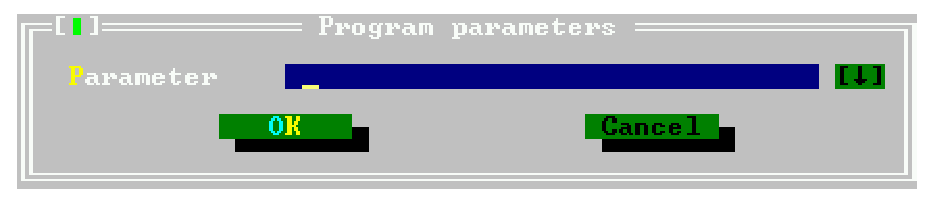
\epsfig{file=pics/ide/params.png,width=\textwidth}
\else
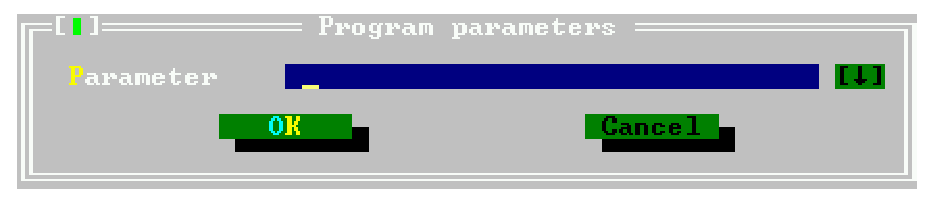
\epsfig{file=pics/ide/params.eps,width=\textwidth}
\fi
\end{figure}
\end{latexonly}

Once the program started, it will continue to run, until 
\begin{enumerate}
\item the program quits normally,
\item an error happens,
\item A breakpoint is encountered.
\end{enumerate}
The last alternative is only possible if the program is compiled
with debug information.

Alternatively, it is possible to position the cursor somewhere in a
source file, and run the program till the execution reaches the
source-line where the cursor is located. This can be done by
\begin{enumerate}
\item selecting "Run|Goto Cursor" in the menu,
\item pressing \key{F4}.
\end{enumerate}
Again, this is only possible if the program was compiled with debug
information.

The program can also executed line by line. Pressing \key{F8} will 
execute the next line of the program. If the program wasn't started
yet, it is started. Repeatedly pressing \key{F8} will execute line 
by line of the program, and the IDE will show the line to be executed 
in an editor window. If somewhere in the code a call occurs to a subroutine,
then pressing \key{F8} will cause the whole routine to be executed before
control returns to the IDE. If the code of the subroutine should be stepped
through as well, then \key{F7} should be used instead. Using \key{F7} will
cause the IDE to execute line by line of any subroutine that is encountered.

If a subroutine is being stepped through, then the "Run|Until return" menu
will execute the program till the current subroutine ends. 

If the program should be stopped before it quits by itself, then this can be
done by
\begin{enumerate}
\item selecting "Run|Program reset" from the menu, or
\item pressing \key{Ctrl-F2}.
\end{enumerate}
The running program will then be aborted.

%%%%%%%%%%%%%%%%%%%%%%%%%%%%%%%%%%%%%%%%%%%%%%%%%%%%%%%%%%%%%%%%%%%%%%%
% Debugging programs
\section{Debugging programs}
\label{se:debugging}
To debug a program, it must be compiled with debug information. Compiling a
program with debug information allows to:
\begin{enumerate}
\item Execute the program line by line.
\item Run the program till a certain point (a breakpoint)
\item Inspect the contents of variables or memory locations while the
program is running.
\end{enumerate}

\subsection{Using breakpoints}
Breakpoints will cause a running program to stop when the execution
reaches the line where the breakpoint was set. At that moment, control
is returned to the IDE, and it is possible to continue execution.

To set a breakpoint,


%%%%%%%%%%%%%%%%%%%%%%%%%%%%%%%%%%%%%%%%%%%%%%%%%%%%%%%%%%%%%%%%%%%%%%%
% The tools menu
\section{The tools menu}
\label{se:toolsmenu}
The tools menu allows you an easy access to external tools. Further,
it contains two other probaly helpful tools for programmers: an
ascii table and a calculator.

\subsection{The messages window}
\label{se:toolsmessages}
The output of the external utilies is redirected by the IDE and it
will be displayed in the message window. The message window is
displayed automatically, if an external tool was run. The
messages window can be also display manual by the selecting the
menu item \var{Tools|Messages} or by pressing the key \key{F11}.

If the output of the tools contains filenames and line numbers,
you can goto the source line by pressing \key{Enter} or
double clicking the output line. To trace the source, press
\key{Space}. The difference between goto and tracking is that
goto closes the message window while tracking keeps the message
window active and the source file is displayed only in the background.

The algorithm which extracts the file names and line numbers from
the tool output is quite sophisticated, but in some cases it may
fail. In this case, please refer the sources of the IDE.

\subsection{GREP}
\label{se:grep}
One external tool in the Tools menu is already predefined: an
menu item to call the \file{grep} utility (\var{Tools|Grep} or
\key{Shift-F2}). \file{grep} search for a given string in files and
returns the lines which contain the string. The search string can
be even a regular expression (see \sees{regexpr}).

\subsection{The ascii table}
\label{se:asciitable}
The tools menu provides also an ascii table (\var{Tools|Ascii table},
it allows you to lookup ascii codes as well as
inserting chars into the window which was active when calling the
ascii chart. To get the ascii code of a char move the blocking block
cursor on this char or click with the mouse on it. To insert a
char into an editor window, double click it with the mouse
or press \key{Enter} while the cursor is on it.

\subsection{The calculator}
\label{se:calculator}
The calculator allows you to do quickly some calculations. It doesn't
take care of operator precedence, so be careful. For more information
about the supported operations, see table \seet{calculatorcommands}.

\begin{FPCltable}{p{5cm}lll}{Calculator commands}{calculatorcommands}
Operation & Button & Key \\
\hline
Add two numbers & \var{+} & \key{+} \\
Subtract two numbers & \var{\-} & \key{\-} \\
Multiply two numbers & \var{*} & \key{*} \\
Divide two numbers & \var{/} & \key{/} \\
Calculate power & \var{x\^y} & \\
Add the displayed number to the memory & \var{M+} & \\
Subtract the displayed number from the memory & \var{M-} & \\
Move the memory contents to the display & \var{M->} & \\
Move the display contents to the memory & \var{M<-} & \\
Exchange display and memory contents & \var{M<->} & \\
Square the display contents & \var{x\^2} & \\
Calculate the reciproke value & \var{1/x} & \\
Calculate the square root & \var{sqr} & \\
Calulate the natural logarithm &  \var{log} & \\
Delete the last typed digit & \var{<-} & \key{Backspace} \\
Delete the display & \var{C} & \key{C} \\
Change the sign & \var{+\-} & \\
Get result of operation & \var{=} & \key{Enter} \\
Do per cent calculation & \var{\%} & \key{\%}
\end{FPCltable}

\subsection{Adding new tools}
\label{se:addingtools}
%%%!!!!!!!!!!!!!!

\subsection{Meta parameters}
When specifing the command line for the called tool, meta parameters can
be used. Meta parameters are variables and and they are replaced
by it's contents before passing the command line to the tool.

%%%!!!!!!!!!!!!!!
\begin{description}
\item[\$CAP]
\item[\$CAP\_MSG]
\item[\$CAP\_EDIT]
\item[\$COL] replaced by the coloumn of the cursor in the active window
\item[\$CONFIG]
\item[\$DIR]
\item[\$DRIVE]
\item[\$EDNAME]
\item[\$EXENAME]
\item[\$EXT]
\item[\$LINE] replaced by the line number of the cursor in the active window
\item[\$NAME]
\item[\$NAMEEXT]
\item[\$NOSWAP]
\item[\$DRIVE]
\item[\$PROMPT]
\item[\$SAVE]
\item[\$SAVE\_ALL]
\item[\$SAVE\_CUR]
\item[\$SAVE\_PROMPT]
\item[\$WRITEMSG]
\end{description}

\subsection{Building your own tool command line dialog box}
%%%!!!!!!!!!!!!!!

%%%%%%%%%%%%%%%%%%%%%%%%%%%%%%%%%%%%%%%%%%%%%%%%%%%%%%%%%%%%%%%%%%%%%%%
% Project management
\section{Project management}
\label{se:projectmanagement}
Luckily, project mangament in pascal is much easier than with C. The
compiler knows from the source which units, sources etc. it needs.
So the \fpc IDE does not need a full featured project manager like
some C development environments offer. But some things make life easier...

\subsection{The primary file}
\label{se:primaryfile}
Without a primary file the IDE compiles/runs the source of the actived
window when you start your program. If you have specified a primary
file, the IDE compiles/runs always this source, no matter if another
source window is active. Select the menu item \var{Compile|Primary file...}
to get a file dialog where you can enter the primary file. Only the command
\var{Compile|Compile} compiles still the active window, this is usefull
if you have a large project and you want only check the syntax of the
current source.

The menu item \var{Compiler|Clear primary file} restores the default behavior
i.e. the compile and run commands apply to the active window.

\subsection{The switches mode}
\label{se:compilermode}
The IDE allows you to work with three different sets of compiler
switches: Normal, Debug and Release. The different switch
sets can be selected in the \var{Switches Mode} dialog which
is executed by the menu item \var{Options|Mode...}.
Change the switches mode doesn't do any active switch change, i.e.
the debug mode doesn't include debug information automatically,
it just loads another set of switches which were adjusted before
by the user in the compiler or directory dialog.

\subsection{The directory dialog}
In the directory dialog, you've to specify the directories where
the compiler should look for units, library etc, where the
output files should be stored etc. You can specify multiple
directories (except for the output directory) seperated by
semicolon.

\begin{description}
\item Nothing yet !!!!!!!!!!!!!!
\end{description}

\subsection{The target operating system}
The menu item \var{Compile|Target} allows you to specify the target
operating system. Changing the target doesn't affect any compiler
switches or directories.

\subsection{The configuration files}
%%%!!!!!!!!!!!!!!

%%%%%%%%%%%%%%%%%%%%%%%%%%%%%%%%%%%%%%%%%%%%%%%%%%%%%%%%%%%%%%%%%%%%%%%
% Customize the IDE
\section{Customize the IDE}
The IDE is configurable in a wide range, you can change colors, screen
resolution etc. The configuration setting can reached via the
submenu \var{Environment} in the \var{Options} menu.

\subsection{Preferences}
The \emph{preferences dialog} is called by the menu item
\var{Options|Environment|Preferences}.

%%%!!!!!!!!!!!!!!

\subsubsection{Video modes}
The \emph{drop down list} at the top of the dialog allows you
to select a video mode.

\begin{remark}
You have to select the video mode by pressing space or clicking
on it. If the drop down list is opened while leaving the dialog,
the new video mode will not be applied.
\end{remark}

The available video modes depend on the system on which the IDE
is running. 

\begin{remark}
If you're using VESA modes under DOS, the display refresh rate may be
annoying low. On older graphics card (1998 and before),
you can try to use the \emph{UniVBE} driver of \emph{SciTech}. But
it is quite outdated (last update somewhere in 1998). For newer
graphics cards which support VESA 3.0, you can try to get one
of the TSR programs
\footnote{\textbf{T}erminate and \textbf{S}tay \textbf{R}esisdent}
available at the net to customize the refresh rate.
%%%%!!!!!!!! footnote with URL
\end{remark}

\subsection{Mouse}
\label{se:prefmouse}
The \emph{mouse options dialog} is called by the menu item
\var{Options|Environment|Mouse}. You can use the slider to adjust the
double clock speed. If you're left handed you can exchange the
behavior of the left and right mouse button by checking the checkbox
item \var{Reverse mouse buttons}.

The two lists with the radio buttons allows you
to configure the behavior of the
right mouse button, if it is clicked together while
pressing the \key{Ctrl} or
\key{Alt} key in an edit window.

The following actions can be assigned to \key{Ctrl}-right mouse button or
\key{Alt}-right mouse button:

\begin{description}
\item [Topic search] The keyword at the mouse cursor is searched in the
help index
\item [Go to cursor] The program is executed until the line where
the mouse cursor is located
\item [Breakpoint] Set a breakpoint at the mouse cursor position
\item [Evalute] Evaluate the value of the variable at the mouse
cursor
\item [Add watch] Add the variable at the mouse cursor to the
watch window
\item [Browse symbol] The symbol at the mouse cursor is displayed
by the browser
\end{description}


%%%%%%%%%%%%%%%%%%%%%%%%%%%%%%%%%%%%%%%%%%%%%%%%%%%%%%%%%%%%%%%%%%%%%%%
% Trouble shooting
\section{Trouble shooting}
%%%!!!!!!!!!!!!!!

%%%%%%%%%%%%%%%%%%%%%%%%%%%%%%%%%%%%%%%%%%%%%%%%%%%%%%%%%%%%%%%%%%%%%%%
% Regular expressions
\section{Regular expressions}
\label{se:regexpr}
A regular expression is a string with sepcial characters which describes 
a whole class of expressions. You may know this from the command line
where can enter a \file{ls *.pas} (or \file{dir *.pas}) to get a list
of all pascal files in a directory. \file{*.pas} is something 
similiar to regular expression. It uses a wildcard to describe a whole 
class of strings: these which end with "\file{.pas}". The possibilty 
of the wildcards in the command line are especially on DOS very limited. 
Regular expressions offer much more: for example \file{[A-Z][0-9]+} 
describes all strings which begin with a upper case letter followed by
one or more digits (you'll understand this regular expression later).

%%%!!!!!!!!!!

%%%%%%%%%%%%%%%%%%%%%%%%%%%%%%%%%%%%%%%%%%%%%%%%%%%%%%%%%%%%%%%%%%%%%%%
% Keyboard shortcuts
\section{Keyboard shortcuts}
\label{se:keyshortcuts}

A lot of keyboard shortcuts used by the IDE are compatible with 
WordStar and should be well known to Turbo Pascal users.

\begin{FPCltable}{p{5cm}ll}{General}{shortcutsgeneral}
Command & Key shortcut & Alternative \\
\hline
Help & \key{F1} & \\
Goto last help topic & \key{Alt-F1} & \\
Search word at cursor position in help & \key{Ctrl-F1} & \\
Help index & \key{Shift-F1} & \\
Close active window & \key{Alt-F3} & \\
Zomm/Unzoom window & \key{F5} & \\
Move/Zoom active window & \key{Ctrl-F5} & \\
Switch to next window & \key{F6} & \\
Switch to last window & \key{Shift-F6} & \\
Menu & \key{F10} & \\
Local menu & \key{Alt-F10} & \\
List of windows & \key{Alt-0} & \\
Active another window & \key{Alt-<digit>} & \\
Call \var{GREP} utility & \key{Shift-F2} & \\
Exit IDE & \key{Alt-X} & \\
\end{FPCltable}
%%%%%%%%%%%%%%%%%%%%%%%%%%%%%%%%%%%%%%%%%%%%%%%%%%%%%%%%%%%%%%%%%%%%%%%%%%%%
\begin{FPCltable}{p{5cm}ll}{Compiler}{shortcutscompiler}
Command & Key shortcut & Alternative \\
\hline
Reset debugger/program & \key{Ctrl-F2} & \\
Display call stack & \key{Ctrl-F3} & \\
Run til cursor & \key{F4} & \\
Switch to user screen & \key{Alt-F5} & \\
Trace into & \key{F7} & \\
Add watch & \key{Ctrl-F7} & \\
Step over & \key{F8} & \\
Set breakpoint at current line & \key{Ctrl-F8} & \\
Make & \key{F9} & \\
Run & \key{Ctrl-F9} & \\
Compile the active source file & \key{Alt-F9} & \\
Message & \key{F11} & \\
Compiler messages & \key{F12} & \\
\end{FPCltable}
%%%%%%%%%%%%%%%%%%%%%%%%%%%%%%%%%%%%%%%%%%%%%%%%%%%%%%%%%%%%%%%%%%%%%%%%%%%%
\begin{FPCltable}{p{5cm}ll}{Text navigation}{shortcutstextnavigation}
Command & Key shortcut & Alternative \\
\hline
Char left & \key{Arrow left} & \key{Ctrl-S} \\
Char right & \key{Arrow right} & \key{Ctrl-D} \\
Line up & \key{Arrow up} & \key{Ctrl-E} \\
Line down & \key{Arrow down} & \key{Ctrl-X} \\
Word left & \key{Ctrl-Arrow left} & \key{Ctrl-A} \\
Word right & \key{Ctrl-Arror right} & \key{Ctrl-F} \\
Scroll one line up & \key{Ctrl-W} & \\
Scroll one line down & \key{Ctrl-Z} & \\
Page up & \key{PageUp} & \key{Ctrl-R} \\
Page down & \key{PageDown} & \\
Beginning of Line & \key{Pos1} & \key{Ctrl-Q-S} \\
End of Line & \key{End} & \key{Ctrl-Q-D} \\
First line of window & \key{Ctrl-Pos1} & \key{Ctrl-Q-E} \\
Last line of window & \key{Ctrl-End} & \key{Ctrl-Q-X} \\
First line of file & \key{Ctrl-PageUp} & \key{Ctrl-Q-R} \\
Last line of file & \key{Ctrl-PageDown} & \key{Ctrl-Q-C} \\
Last cursor position & \key{Ctrl-Q-P} & \\
\end{FPCltable}
%%%%%%%%%%%%%%%%%%%%%%%%%%%%%%%%%%%%%%%%%%%%%%%%%%%%%%%%%%%%%%%%%%%%%%%%%%%%
\begin{FPCltable}{p{5cm}ll}{Edit}{shortcutsedit}
Command & Key shortcut & Alternative \\
\hline
Delete char & \key{Del} & \key{Ctrl-G} \\
Delete left char & \key{Backspace} & \key{Ctrl-H} \\
Delete line & \key{Ctrl-Y} & \\
Delete til end of line & \key{Ctrl-Q-Y} & \\
Delete word & \key{Ctrl-T} & \\
Insert line & \key{Ctrl-N} & \\
Toggle insert mode & \key{Insert} & \key{Ctrl-V} \\
\end{FPCltable}
%%%%%%%%%%%%%%%%%%%%%%%%%%%%%%%%%%%%%%%%%%%%%%%%%%%%%%%%%%%%%%%%%%%%%%%%%%%%
\begin{FPCltable}{p{5cm}ll}{Block commands}{shortcutsblockcommands}
Command & Key shortcut & Alternative \\
\hline
Goto Beginning of selected text & \key{Ctrl-Q-B} & \\
Goto end of selected text & \key{Ctrl-Q-K} & \\
Select current line & \key{Ctrl-K-L} & \\
Print selected text & \key{Ctrl-K-P} & \\
Select current word & \key{Ctrl-K-T} & \\
Delete selected text & \key{Ctrl-Del} & \key{Ctrl-K-Y} \\
Copy selected text to cursor position & \key{Ctrl-K-C} & \\
Move selected text to cursor position & \key{Ctrl-K-V} & \\
Copy selected text to clipboard & \key{Ctrl-Ins} & \\
Move selected text to the clipboard & \key{Shift-Del} & \\
Indent block one coloumn & \key{Ctrl-K-I} & \\
Unindent block one coloumn & \key{Ctrl-K-U} & \\
Insert text from clipboard & \key{Shift-Insert} & \\
Insert file & \key{Ctrl-K-R} & \\
Write selected text to file & \key{Ctrl-K-W} & \\
\end{FPCltable}
%%%%%%%%%%%%%%%%%%%%%%%%%%%%%%%%%%%%%%%%%%%%%%%%%%%%%%%%%%%%%%%%%%%%%%%%%%%%
\begin{FPCltable}{p{5cm}ll}{Change selection}{changeselection}
Command & Key shortcut & Alternative \\
\hline
Mark beginning of selected text & \key{Ctrl-K-B} & \\
Mark end of selected text& \key{Ctrl-K-K} & \\
Remove selection & \key{Ctrl-K-H} & \\
Extend selection one char to the left & \key{Shift-Arrow left} & \\
Extend selection one char to the right & \key{Shift-Arrow right} & \\
Extend selection to the beginning of the line & \key{Shift-Pos1} & \\
Extend selection to the end of the line & \key{Shift-End} & \\
Extend selection to the same coloumn in the last row & \key{Shift-Arrow up} & \\
Extend selection to the same coloumn in the next row & \key{Shift-Arrow down} & \\
Extend selection to the end of the line & \key{Shift-End} & \\
Extend selection one word to the left & \key{Ctrl-Shift-Arrow left} & \\
Extend selection one word to the right & \key{Ctrl-Shift-Arrow right} & \\
Extend selection one page up & \key{Shift-PageUp} & \\
Extend selection one page down & \key{Shift-PageDown} & \\
Extend selection to the beginning of the file & \key{Ctrl-Shift-Pos1} &
\key{Ctrl-Shift-PageUp} \\
Extend selection to the end of the file & \key{Ctrl-Shift-End} &
\key{Ctrl-Shift-PageUp} \\
\end{FPCltable}
%%%%%%%%%%%%%%%%%%%%%%%%%%%%%%%%%%%%%%%%%%%%%%%%%%%%%%%%%%%%%%%%%%%%%%%%%%%%
\begin{FPCltable}{p{5cm}ll}{Misc. commands}{shortcutsmisccommands}
Command & Key shortcut & Alternative \\
\hline
Save file & \key{F2} & \key{Ctrl-K-S} \\
Open file & \key{F3} & \\
Search & \key{Ctrl-Q-F} & \\
Search again & \key{Ctrl-L}\ & \\
Search and replace & \key{Ctrl-Q-A} & \\
Set mark & \key{Ctrl-K-n} (where n can be 0..9) & \\
Goto mark & \key{Ctrl-Q-n} (where n can be 0..9) & \\
Undo & \key{Alt-Backspace} & \\
\end{FPCltable}
%
%  $Log$
%  Revision 1.1.2.4  2000-11-15 18:58:35  michael
%  + Debug continued
%
%  Revision 1.1.2.3  2000/11/14 23:24:09  michael
%  + Documented run menu
%
%  Revision 1.1.2.2  2000/11/13 23:46:03  michael
%  + documented blocks, search, and the browser
%
%  Revision 1.1.2.1  2000/11/12 23:40:32  michael
%  + Changes for final version
%
%  Revision 1.1  2000/07/13 09:10:04  michael
%  + Initial import
%
%  Revision 1.5  2000/03/04 07:47:28  florian
%    * some corrections and some new stuff
%
%  Revision 1.4  2000/03/01 15:39:40  florian
%    * some new stuff
%
%  Revision 1.3  2000/02/28 17:45:40  florian
%    * a lot of new stuff
%